\documentclass{letter}

\usepackage{csquotes}
\usepackage[margin=1in]{geometry}
\usepackage{tikz}
\usepackage{amsmath}
\usepackage{enumerate}

\newcommand{\heading}[1]{{\large \textsc{#1}}}

\begin{document}

\heading{COMP 282 - Midterm 1 (Spring, 2019)}
\kern 2cm
\heading{Name:}

{\bf Question 1 (10 Points)} \kern 0.5cm Provide a short answer to the following
questions.

\begin{enumerate}[a]

\item Give an example of when you might use a linked list.

\vspace{3cm}

\item Give an example of when you would use a graph.

\vspace{3cm}

\item What is the property that allows Binary Trees to be quickly searchable?
What is an ``easy'' way of maintaining this property?

\vspace{3cm}

\item We know that all trees are graphs.  Why are not all graphs trees?

\vspace{3cm}

\item Why do we have asyptotic analysis (Big-O notation)?

\end{enumerate}

\clearpage

{\bf Question 2 (10 Points)} \kern 0.5cm Circle the appropriate choices for the
following questions.  There may be more than one correct answer.

\begin{enumerate}[a]

\item Which data structures are searchable in $O(\lg n)$ time.  Assume any
favorable arrangements of data necessary to achieve this property.

\begin{enumerate}[i]

\item Trees
\item Linked Lists
\item Arrays
\item Graphs
\item Binary Trees
\item None of These

\end{enumerate}

\vspace{0.5cm}

\item Of these, which is the most appropriate data structure with which to
construct a FIFO queue?

\begin{enumerate}[i]

\item Trees
\item Arrays
\item Primitive
\item Binary Trees
\item Linked Lists

\end{enumerate}

\vspace{0.5cm}

\item Which of the following properties are relevant to binary trees?

\begin{enumerate}[i]

\item Balance
\item Mass Density
\item Edge Weight
\item Shortest Path
\item Height
\item Half-Life

\end{enumerate}

\vspace{0.5cm}

\item Circle both the {\em minimum} and {\em maximum} height a binary tree
containing 31 values may have.

\begin{enumerate}[i]

\item 0
\item 31
\item 6
\item 42
\item 5
\item 4

\end{enumerate}

\end{enumerate}

\clearpage

{\bf Question 3 (10 Points)} \kern 0.5cm Given the following scenarios,
describe a data structure that would be most-appropriate.  Justify each.

\begin{enumerate}[a]

\item You are building an e-commerce site which is expected to have a lot daily
visitors.  The problem is, your payment system is notoriously slow to process
individual payments.  You want a way to keep track of all customers currently
waiting to check out their orders.

\vspace{8cm}

\item You are writing a program for the campus library.  The task is to
organize all the Computer Science research papers currently in the archives.
Each article has a list of references at the end that refer to other articles
in the collection.

\end{enumerate}

\clearpage

{\bf Question 4 (10 Points)} \kern 0.5cm Provide all of the listed traversals for
the following binary tree.  Be sure to label them.

\begin{itemize}
\item Pre-order traversal.
\item In-order traversal.
\item Breadth-first traversal.
\end{itemize}

\begin{center}
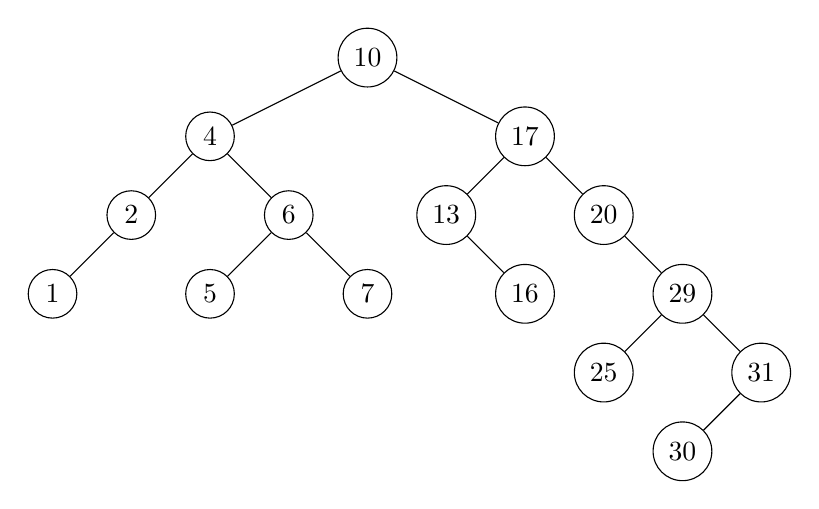
\begin{tikzpicture}
\node[shape=circle,draw=black] (10) at (0,0) {10};
\node[shape=circle,draw=black] (4) at (-2,-1) {4};
\node[shape=circle,draw=black] (6) at (-1,-2) {6};
\node[shape=circle,draw=black] (2) at (-3,-2) {2};
\node[shape=circle,draw=black] (5) at (-2,-3) {5};
\node[shape=circle,draw=black] (7) at (0,-3) {7};
\node[shape=circle,draw=black] (1) at (-4,-3) {1};
\node[shape=circle,draw=black] (17) at (2,-1) {17};
\node[shape=circle,draw=black] (13) at (1,-2) {13};
\node[shape=circle,draw=black] (20) at (3,-2) {20};
\node[shape=circle,draw=black] (16) at (2,-3) {16};
\node[shape=circle,draw=black] (29) at (4,-3) {29};
\node[shape=circle,draw=black] (25) at (3,-4) {25};
\node[shape=circle,draw=black] (31) at (5,-4) {31};
\node[shape=circle,draw=black] (30) at (4,-5) {30};

\path (10) edge (4);
\path (4) edge (6);
\path (4) edge (2);
\path (6) edge (5);
\path (6) edge (7);
\path (2) edge (1);
\path (10) edge (17);
\path (17) edge (13);
\path (17) edge (20);
\path (13) edge (16);
\path (20) edge (29);
\path (29) edge (25);
\path (29) edge (31);
\path (31) edge (30);
\end{tikzpicture}
\end{center}

\clearpage

{\bf Question 5 (20 Points)} \kern 0.5cm Use Kruskal's Algorithm to calculate the
minimum spanning forest of the following graph $G = (V, E, w)$.  Show all
steps.  List all vertices in a particular spanning tree, and give its final
cost.

\begin{equation*}
V = \left \{ v_0, v_1, v_2, v_3, v_4, v_5, v_6, v_7, v_8, v_9 \right \}
\end{equation*}

\begin{tabular}{ c | c }
E & w \\ \hline
$\{v_0,v_1\}$ & 3 \\
$\{v_1,v_2\}$ & 2 \\
$\{v_3,v_4\}$ & 3 \\
$\{v_4,v_5\}$ & 1 \\
$\{v_5,v_6\}$ & 2 \\
$\{v_6,v_4\}$ & 2 \\
$\{v_6,v_7\}$ & 4 \\
$\{v_7,v_4\}$ & 3 \\
$\{v_7,v_8\}$ & 2 \\
$\{v_8,v_9\}$ & 1 \\
$\{v_9,v_5\}$ & 4 \\
\end{tabular}

\clearpage

{\bf Question 6 (20 Points)} \kern 0.5cm Given the following graph $G=(V,E)$, use
any (appropriate) algorithm discussed in class to list the vertices that form a
connected component with $v_3$.  State the algorithm you are using, show all
steps.

\begin{equation*}
V = \left \{ v_0, v_1, v_2, v_3, v_4, v_5, v_6, v_7, v_8, v_9 \right \}
\end{equation*}
\begin{equation*}
E = \left \{ \{v_0,v_1\},\{v_1,v_4\},\{v_3,v_2\},\{v_2,v_5\},\{v_5,v_6\},\{v_5,v_8\},\{v_6,v_8\},\{v_6,v_9\},\{v_7,v_6\},\{v_8,v_7\},\{v_7,v_9\},\{v_9,v_8\} \right \}
\end{equation*}

\clearpage

{\bf Question 7 (20 Points)} \kern 0.5cm Given the graph $G = (V, E, w)$, below,
find the shortest path between $v_2$ and $v_6$.  Show all steps.

\begin{equation*}
V = \{ v_0, v_1, v_2, v_3, v_4, v_5, v_6, v_7, v_8, v_9 \}
\end{equation*}

\begin{tabular}{ c | c }
E & w \\ \hline
$\{v_0,v_4\}$ & 1 \\
$\{v_0,v_1\}$ & 7 \\
$\{v_0,v_6\}$ & 2 \\
$\{v_1,v_2\}$ & 4 \\
$\{v_1,v_0\}$ & 7 \\
$\{v_2,v_9\}$ & 3 \\
$\{v_2,v_8\}$ & 6 \\
$\{v_2,v_7\}$ & 4 \\
$\{v_3,v_2\}$ & 1 \\
$\{v_5,v_2\}$ & 3 \\
$\{v_5,v_6\}$ & 4 \\
$\{v_6,v_2\}$ & 10 \\
$\{v_6,v_7\}$ & 2 \\
\end{tabular}

\clearpage

\end{document}
